\subsection{Shared state: \textit{libgotcha}}
\label{sec:libgotcha}

Our discussion of libinger's implementation was complete but for one important
detail:\@ shared state.  As described so far, the library provides an interface that
makes it unsafe to call functions that are not async-signal safe after the
\texttt{launch()} call site.  Fortunately, users of libinger are spared from this
restriction because it is linked against another library, \textit{libgotcha} that
automatically protects much of a program's shared state.

Before discussing what libgotcha does, it is useful to clarify what it does
\textit{not} do.  Consider Listing~\ref{lst:ingerbug}, which shows
a code passage with a concurrency bug:\@ because the \texttt{timed()} function does
not use an atomic increment operation, its \texttt{launch()} invocation might be
preempted after reading the \texttt{count} variable but before writing it, in which
case the \texttt{resume()} will set the value back to \texttt{1}, causing
the assertion to fail.  Note that this bug is located within a program that makes
explicit use of preemptible functions; for this reason, we deem it to be out of
libgotcha's scope and assign responsibility for avoiding it to the author of that
program, or the language.  Indeed, had the code segment been written in Rust instead
of C, this bug would not be possible:\@ libinger's Rust bindings restrict the
preemptible function to only access access state in a thread-safe manner
(\texttt{Send}).  As such, the compiler would force the programmer to use an atomic
or lock to guard the counter\footnote{Of course, this means it is still possible to
create deadlock or some other logic error, but it does protect against undefined
behavior.}.

\begin{lstlisting}[label=lst:ingerbug,caption=Concurrency bug in internal stateful code]
static int count = 0;

static void *timed(void *ignored) {
	++count;
	return NULL;
}

int main(void) {
	struct linger res = launch(timed, VERY_SHORT, NULL);
	++count;
	resume(&res, LONG_ENOUGH);
	assert(count == 2); // BUG!
	return 0;
}
\end{lstlisting}

We instead focus our efforts on shared state occurring within an object file
(roughly, compilation unit)\footnote{Whenever we refer to an object file, we mean
specifically a relocated object file (i.e., executable or dynamic shared library);
that is, one that is loaded into the process's memory image while a program is
running.  In other words, a ``linking unit'' or ``software project.''} that does not
use preemptible functions.  Our reasoning is that such code cannot be expected to
even be aware of the existence of preemptible functions, and therefore should not be
subject to systemic concurrency concerns resulting from their use.  For instance,
using a nonreentrant libc interface such as \texttt{strtok()} from after
\texttt{launch()} should not break it for the preemptible function.  The task of
libgotcha is to automatically mitigate concurrency considerations between independent
object files in order to allow applications that use preemptible functions to link
against existing third-party shared libraries without recompiling them.

The libgotcha library employs a technique we'll refer to as \textbf{selective
relinking} to redirect at runtime each use of a function or global variable from
outside the current object file to one of a number of possible copies.  The libinger
library leverages this functionality to weaken the semantics of either dynamic
linking or preemption, depending on the symbol being accessed.  In the common case,
we weaken the former by redirecting to a ``personal'' copy of the symbol, thereby
separating any shared state that might become inconsistent from the rest of the
program.  Although this approach works for many libraries, it is sometimes
inappropriate for function calls; for instance, using multiple copies of the dynamic
allocator would cause them to manage the same heap with different free lists.  In
such cases, we instead defer preemption until the function returns.

Specifically, libgotcha presents an API based on something we term a \textbf{libset},
which is a full copy of the program's set of loaded libraries\footnote{Technically, a
libset also includes the executable, which is needed in case one of the application's
libraries uses preemptible functions that use symbols from the executable file.}.
This might be the \textbf{main libset} (the program itself, as originally loaded), or
one of any number of copies that libgotcha opens.  Each thread has an attribute
called the \textbf{current libset} that controls which libset symbol uses are
redirected to.  This does not determine the libset from which the current code is
being executed, but rather the libset that will be switched to upon leaving that
code's object file.  Users of libgotcha may explicitly reinitialize a libset, closing
all its loaded objects then reopening them to prepare for fresh use.

The final feature of libgotcha is a \textbf{whitelist} of symbols (such as the
dynamic allocator) that should share a single definition throughout the entire
application.  Whenever a global variable from this list is accessed, libgotcha serves
the definition from the main libset.  Whenever a function from the list is called,
libgotcha automatically changes the thread's current libset to the main one before
performing the call, then restores its original value as soon as the function
returns.  Users of libgotcha can optionally install a callback function to be
notified whenever the latter libset switch occurs.

One activates the functionality of libgotcha simply by linking against it:\@ once
loaded into the process image, it immediately instruments the boundaries between
object files.  The libinger shared library is statically linked against
libgotcha\footnote{The attentive reader will notice that both libgotcha and libinger
contain shared state (the current libset and thread preemption signal, respectively).
To handle this, libgotcha automatically adds all the symbols defined by its own
object file to the whitelist.  By statically linking to it, libinger gains this same
protection.} so that the latter is active in any program using preemptible functions.

Use of this API by libinger is straightforward.  The \texttt{launch()} function
allocates a new libset by either using an unused one, reusing one from a preemptible
function that ran to completion, or reinitializing one from a preemptible function
that was canceled prematurely\footnote{We assume that any canceled preemptible
function has left its libset in an undefined state.  While libinger currently
performs libset reinitialization synchronously, this somewhat costly step could be
moved off the critical path by assigning a separate reaper thread.}.  It installs
this as the current libset just before enabling preemption.  Right after checking
whether the received signal was intended for the current thread, the preemption
signal handler checks the thread's current libset; in the case of the main one
(indicating the preemptible function is currently in whitelisted code), it blocks the
preemption signal and immediately returns, effectively deferring
preemption\footnote{When whitelisting the dynamic allocator, it is important not to
whitelist all of libc as collateral damage, since preemptible functions could easily
exploit this to run forever (e.g., by performing their work in the \texttt{qsort()}
function's comparator callback).  Fortunately, libc uses dynamic calls when it needs
to invoke the allocator internally, allowing us to whitelist that component alone.}.
The deferral is not indefinite:\@ libinger uses libgotcha's callback mechanism to
both call the handler and unblock the signal as soon as the function returns.
Figure~\ref{fig:callwhitelist} shows the effect of calling \texttt{launch()} on a
preemptible function that calls \texttt{malloc()}.

\begin{figure}
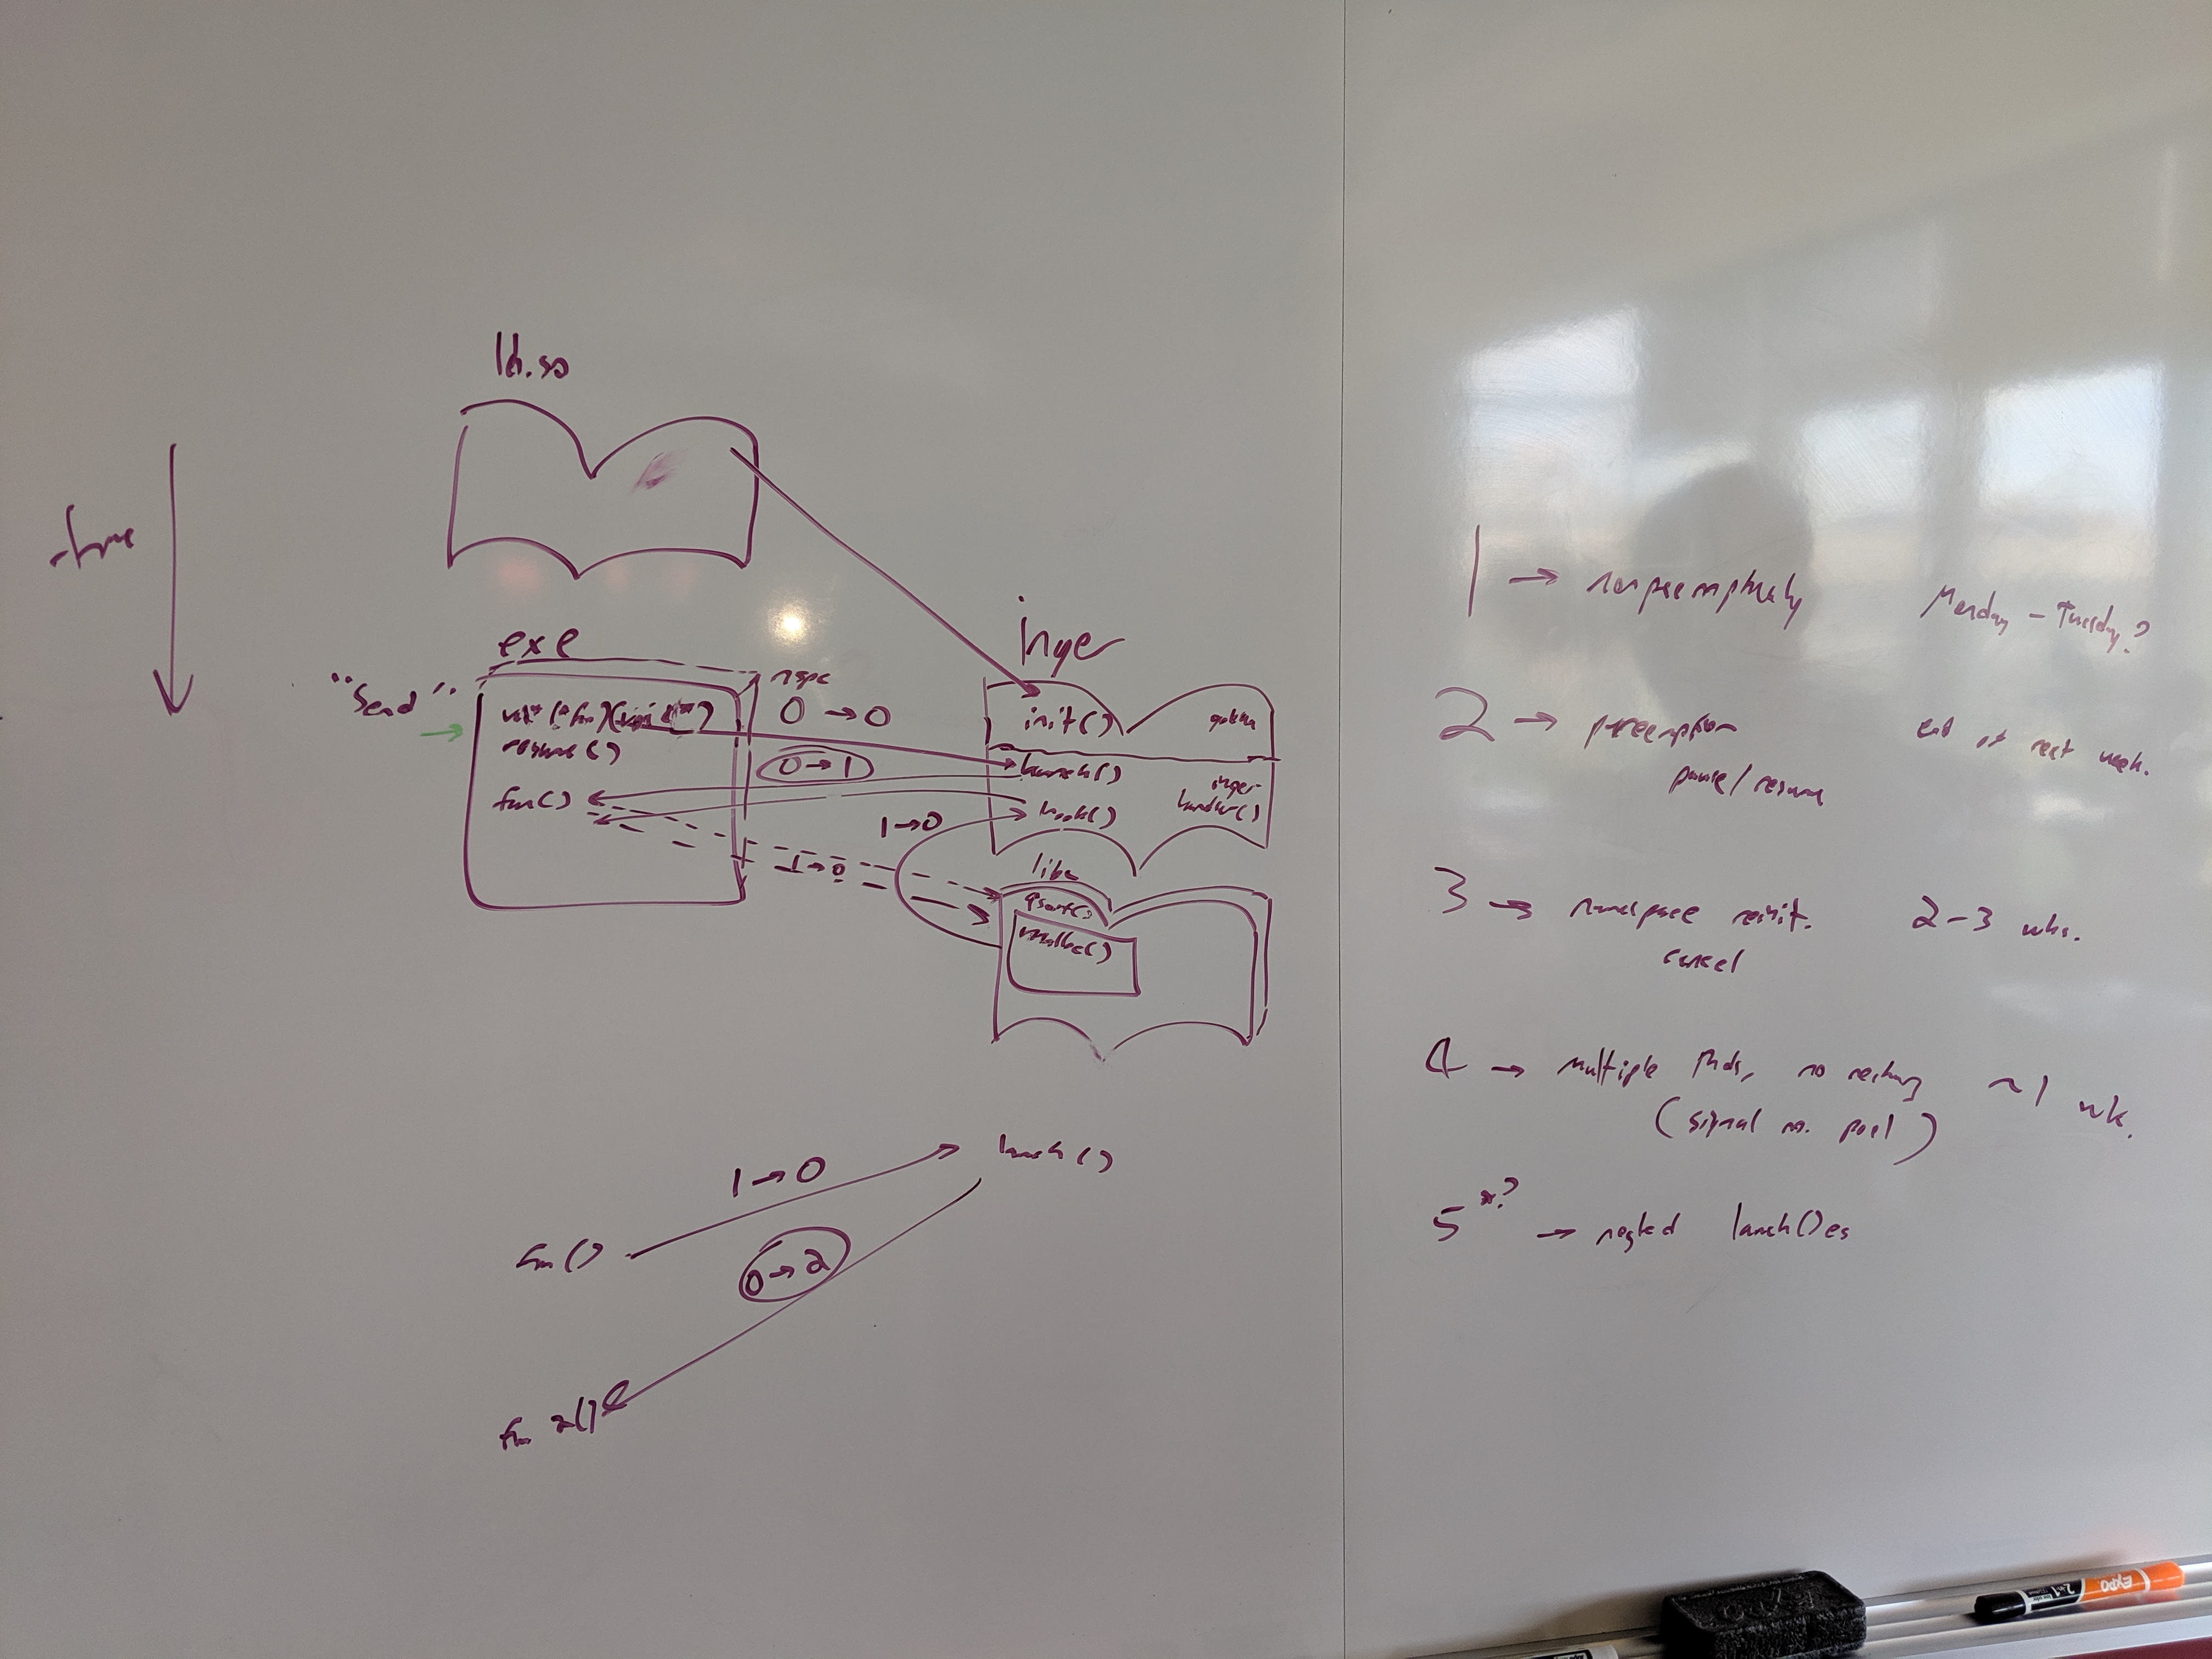
\includegraphics[width=\columnwidth]{figs/calltree}
\caption{How preemptible function dispatch works}
\label{fig:callwhitelist}
\end{figure}

The rest of this section covers the implementation of libgotcha.  We begin with a
brief review of dynamic linking itself.

\paragraph{Dynamic linking}

The key feature of shared libraries is the ability to replace them between the time
an
application is built and when it is executed.  This is enabled by dynamic linking, an
approach by which the static linker delays the relocation of addresses associated
with \textbf{dynamic calls} to functions and \textbf{dynamic references} to global
variables.  Instead of resolving their addresses directly within the output machine
code, the static linker includes a
\textbf{dynamic relocation table} in each output ELF object file describing the
locations of dynamic calls and references, as well as the name of each target symbol.
A component of the C runtime known as the dynamic linker (\texttt{ld.so}) uses this
table to resolve dynamic symbol addresses after the application is loaded.

When a dynamically-linked application is run, the kernel first passes control to the
dynamic linker, which reads its shared library dependencies from the executable's ELF
headers.  It then loads these libraries into the process image, repeats with
\texttt{their} dependencies, and so on.  The linker also provides a \texttt{dlopen()}
that can be used to load additional shared object files at runtime.  The GNU dynamic
linker extends this interface with the Solaris concept of namespaces, each of which
represents an independent dependency graph of loaded libraries.  It is this feature
upon which we build the libset abstraction, which extends this notion of duplicate
copies of a library to allow one namespace's use of a symbol to resolve to a
definition in a different namespace.

It is important to realize that dynamic calls and references are resolved based on
the name of a symbol, which may be ambiguous between multiple libraries within the
same namespace; as such, the library associated with each dynamic relocation is not
determined until runtime.  In fact, a dynamic relocation might even resolve back to
the same object file that contains it; this is most common when a shared library
makes an internal reference to one of its own public interfaces (since the
application might replace that public interface with its own implementation or one
from a different library).  Note that other internal references within such a shared
library are linked statically, leaving no way to locate them at runtime.  In order to
provide consistent semantics, we only instrument \textbf{cross-library} variable
references and function calls, where the use and definition occur in different object
files.

\paragraph{GOTs and PLTs}

When the dynamic linker needs to resolve a symbol use to the address of its
corresponding definition, it looks up the symbol name in the relocation table and
searches the dependency graph of loaded object files for the first definition of a
symbol with that name.  Having found the definition, it needs to store the address
where the program can find it during execution.  Unlike the static linker, it does
not modify the program's executable regions; instead, it places the resolved address
into the requesting object file's \textbf{global offset table (GOT)}\footnote{It is
from this structure that \textit{lib\textbf{got}cha} gets its name.}, a structure
created by the static linker with a spot corresponding to each dynamic relocation.

Dynamic calls to functions are slightly more complicated because they can resolve
lazily at first invocation.  For instance, the instruction
\texttt{call~printf@plt} causes the assembler to generate a corresponding executable
\textbf{procedure linkage table (PLT)} stub function, as shown in
Listing~\ref{lst:plt}.  The first instruction of this stub looks up the address of
the
function by checking a corresponding GOT entry; however, initially this contains the
address of the immediately-following \texttt{pushq} instruction!  Thus, on the first
call, the PLT stub pushes a symbol relocation identifier (here, \texttt{0x0}) onto
the stack and calls into the dynamic linker, which resolves the symbol to the
function's real address, memoizes the result by updating the GOT entry, and finally
jumps into the real function.  Subsequent calls to the PLT stub then forward to the
real function after executing only the initial \texttt{jmpq} instruction.

\begin{lstlisting}[label=lst:plt,caption=Example PLT entry for call to \texttt{printf()}]
0000000000001030 <printf@plt>:
	1030: jmpq  *0x2fe2(%rip) <printf>
	1036: pushq $0x0
	103b: jmpq  1020          <.plt>
\end{lstlisting}

\paragraph{Intercepting cross-library calls}

The libgotcha library includes a constructor that gets invoked by the dynamic linker
after all shared libraries have been loaded but before the call to \texttt{main()}.
Recall that our goal is to reroute cross-library uses of symbols at runtime.  This
means we need to instrument all use sites and inject our own code that can decide
which libset to route to.  In the case of cross-library calls, we have a significant
advantage:\@ each PLT entry already executes by branching to an address stored in the
GOT, so the constructor has only to change the latter to one of its own functions,
and any calls through that PLT entry will be sent to libgotcha instead.

Before updating any GOT entries, we must identify
which ones correspond to cross-library calls.  Doing this is a multi-step process:
First, we traverse the relocation table for each loaded object file, cross
referencing each of its relocation entries against the local object file's symbol
table.  If the symbol table does not contain a definition matching the relocation
entry's target, we conclude that the relocation must correspond to a cross-library
call.  Otherwise, we check the address in the GOT entry corresponding to the
relocation entry:  If this address is outside the bounds of the current object file,
it is a cross-library call.  Otherwise, if this address matches the one from the
symbol table entry, it is not a cross-library call, and should be skipped.  The last
case is the trickiest, since the GOT entry probably still refers to the PLT stub
(because the symbol reference has not yet been resolved).  In this case, we resolve
the symbol
early, update the GOT entry, and recheck whether it resolved to the local definition
to determine whether it is a cross-library call.

Next, the constructor allocates one or more executable pages full of custom PLT-like
stubs, which we refer to as the \textbf{procedure linkage override tables (PLOTs)}.
Each PLOT is associated with one \textbf{shadow GOT} for each namespace:\@ when a
particular PLOT stub is executed, it pushes an index to the stack and calls a
function, \texttt{procedure\_linkage\_override()}, that decides which libset the call
should target, locates the corresponding shadow GOT, and transfers control to the
address listed at the appropriate index in that table.  (Because this function
is injected into the "middle" of function calls, it is written in assembly to avoid
clobbering any of the application's registers.)  The constructor sets up this system
by replacing each GOT entry corresponding to a cross-library call with a fresh PLOT
entry, storing its previous value in the shadow GOT for the main namespace.  It then
opens a fixed number of additional libsets, redirects the cross-library calls from
each new copy of a library to the same PLOT stubs as before, and creates a shadow GOT
for each libset.

The setup procedure described so far has one significant problem:\@ recall that a PLT
call memoizes the real address of its symbol by replacing the GOT entry, which should
cause subsequent calls to skip libgotcha's \texttt{procedure\_linkage\_override()}
codepath.  In order to prevent this, the constructor updates the relocation entries
corresponding to cross-library calls to point at \textit{shadow} GOT entries.  This
fools the dynamic linker into updating the shadow entry instead, meaning that
memoization still works, as shown in Figure~\ref{fig:override}.

\begin{figure}
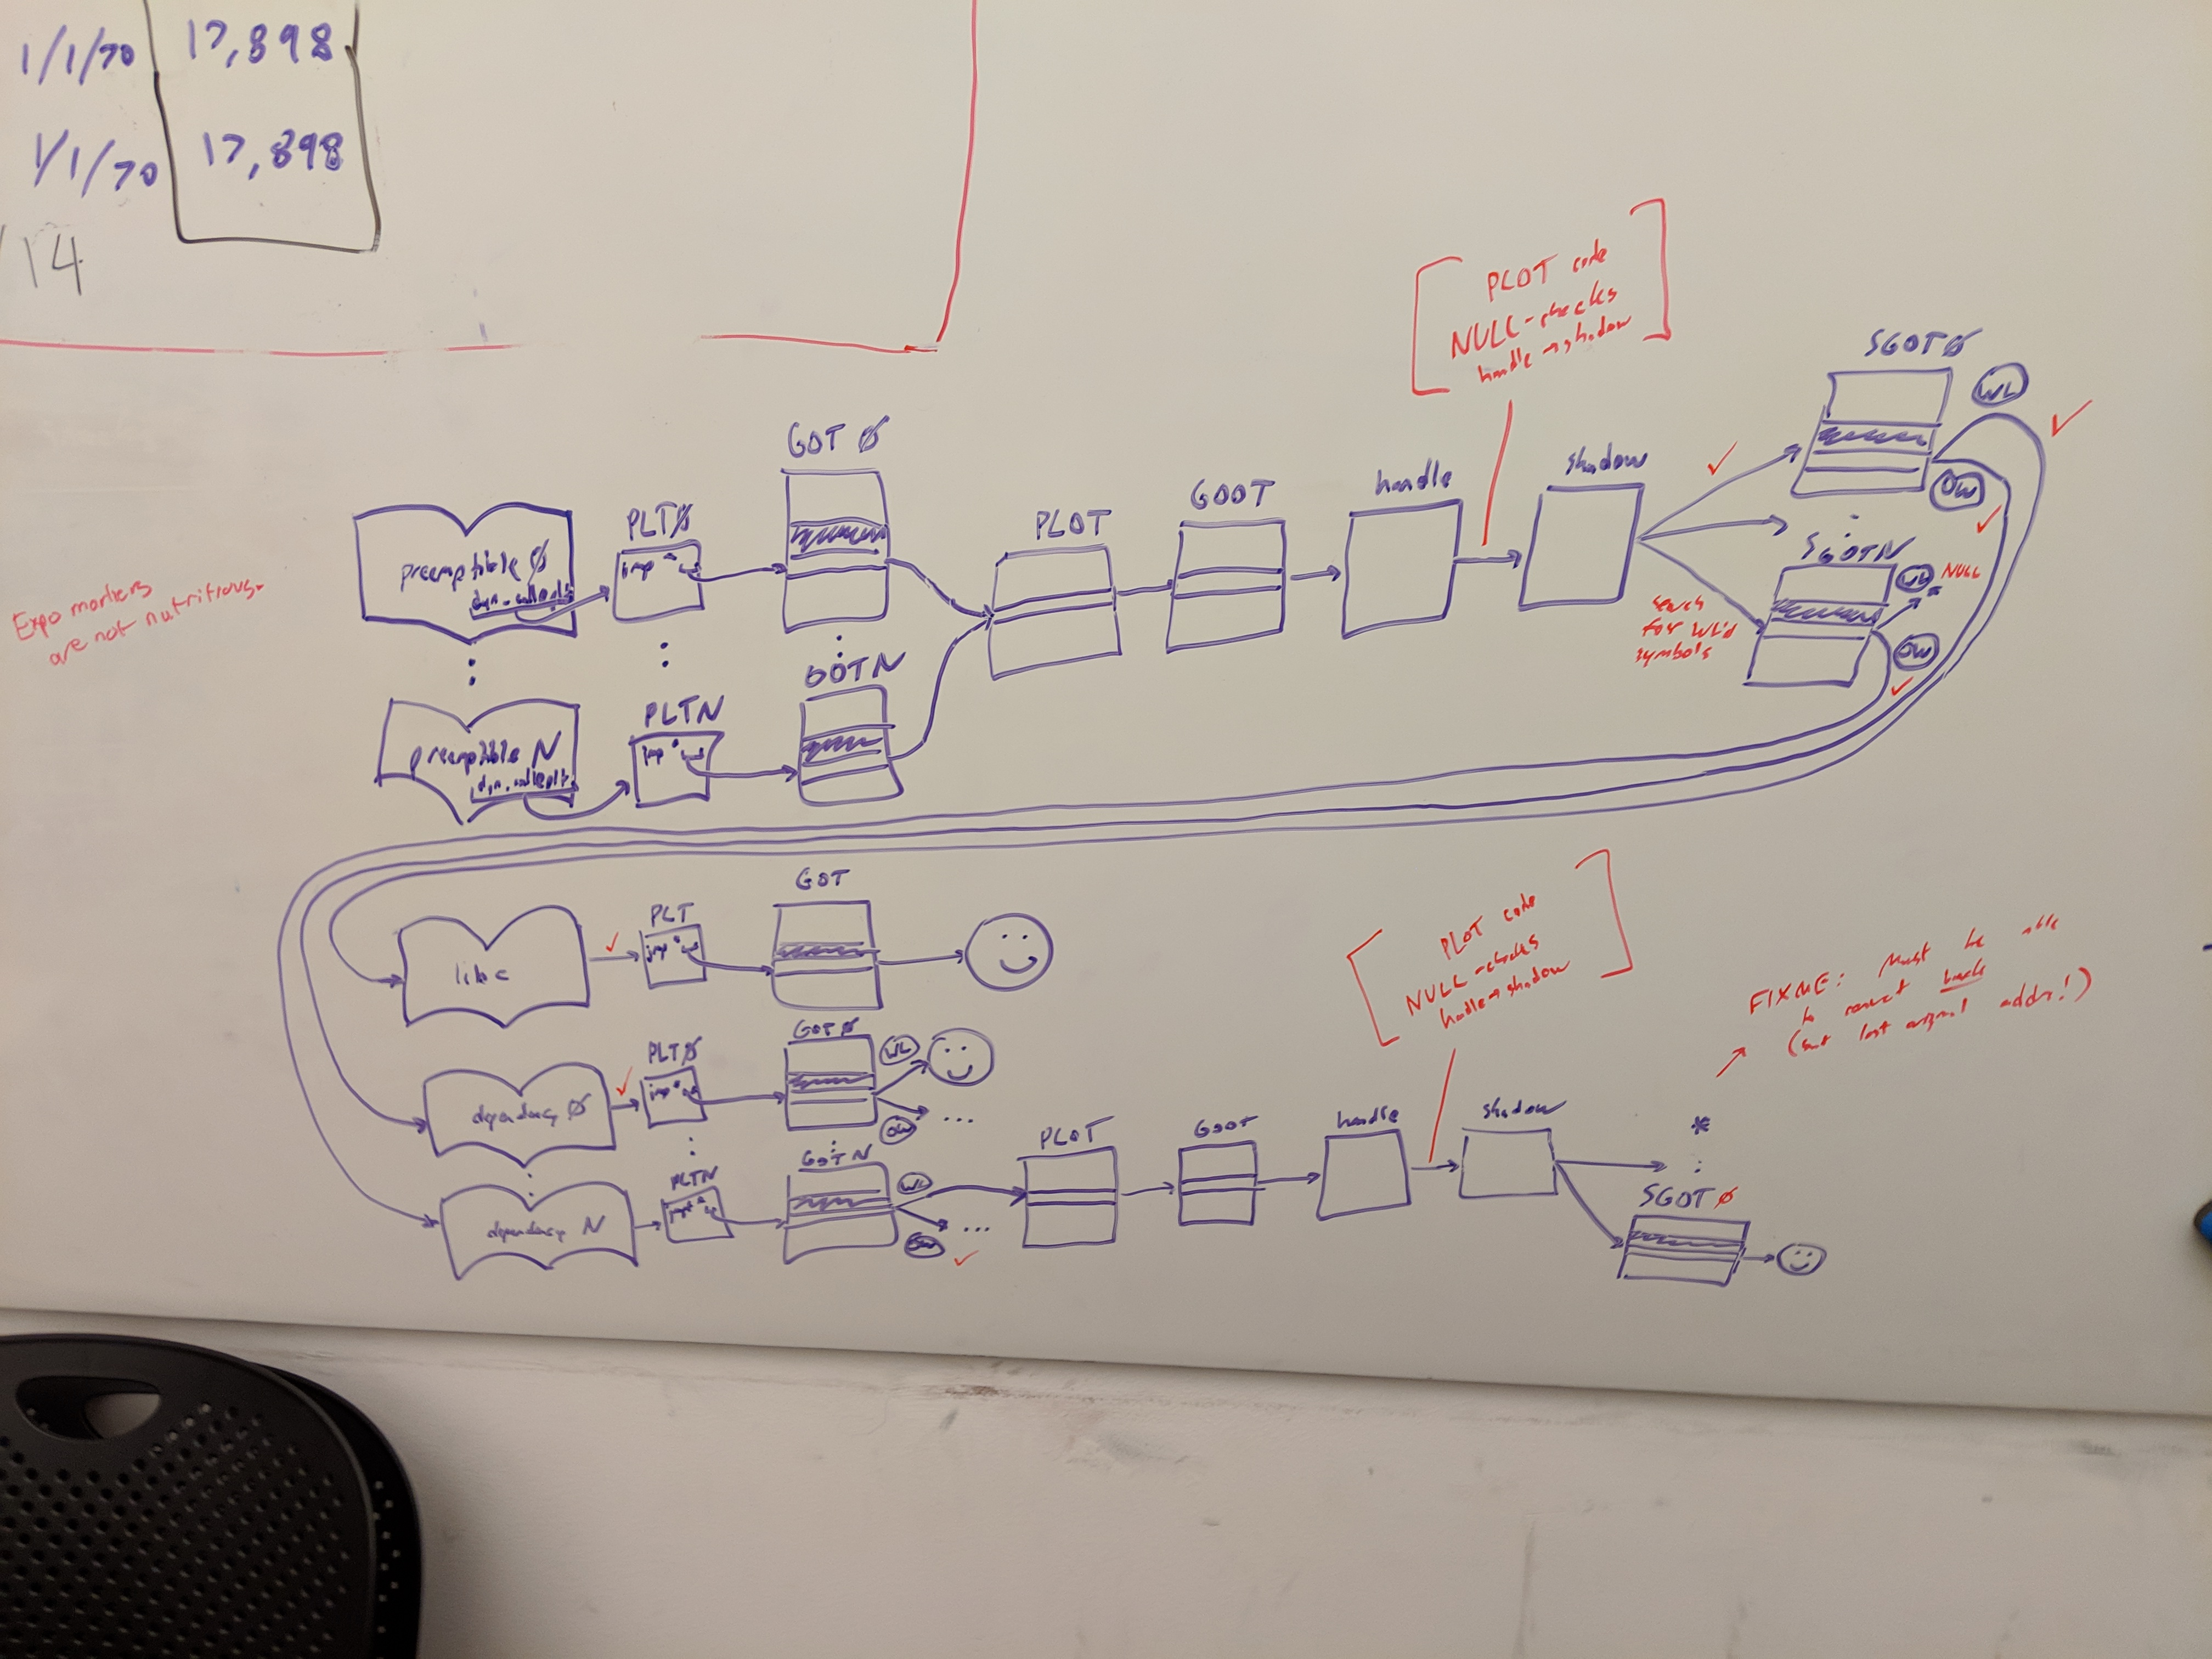
\includegraphics[width=\columnwidth]{figs/tables}
\caption{\texttt{procedure\_linkage\_override()}'s table lookups}
\label{fig:override}
\end{figure}

\paragraph{Incercepting cross-library references}

The reader might notice that invocation is not the only thing a program can do with a
function:\@ it might also pass around the function's address.  In fact, after taking
the address, it could pass it to code within a different object file, which might
compare it\footnote{In order for such comparisons to correctly indicate whether the
same code will be run, the compiler loads such addresses directly from the GOT via
instructions of the special position-independent relocation form
\texttt{mov~\textit{symbol}@gotpcrel(\%rip),~\%\textit{dest}}, and the dynamic linker
resolves the calls and populates their GOT entries eagerly at load time.}.  To avoid
breaking pointer-comparison semantics, libgotcha makes sure to share the same PLOT
stub between all GOT entries to a given symbol that use this type of
relocation.  As long as the current libset remains the same between the time of a
function pointer comparison and the time of its invocation, such a comparison
guarantees that \texttt{procedure\_linkage\_override()} will dispatch to the same
copy when invoked using either pointer.

Handling references to global data besides functions is more challenging, and less
efficient, because such accesses use the aforementioned position-independent
relocation but do not include a PLT-style codepath for us to co-opt.
In order to capture (hopefully rare) cross-library references to global variables,
we use a different approach.  After each shadow GOT page, we allocate an inaccessible
page with no protection bits set.  Each time the libgotcha constructor encounters a
relocation entry corresponding to a data symbol, we migrate the contents of its GOT
entry into an available shadow GOT entry, replacing it with an address the same
number of bytes into the shadow GOT's corresponding inaccessible page\footnote{For
security reasons, the dynamic linker leaves the portion of each GOT corresponding to
eargerly-resolved symbol uses read-only.  We restore write access to these entries
using \texttt{mprotect()}, then remove it again after updating the entries.}.  Thus,
whenever the program takes the address of a particular symbol, it gets the same fake
address.  Any attempt to read from or write to this address results in a segmentation
fault, which libgotcha catches; we then look up the real address in the shadow GOT
corresponding to the currently-selected libset, disassemble the offending
instruction(s), and replace the contents of the memory-address register with the
found address.  Once the signal handler returns, the instruction executes again, this
time with a valid memory address in its register\footnote{Although it is possible to
generate code sequences that are incompatible with this approach (e.g., because they
perform in-place pointer arithmetic on a register rather than using displacement-mode
addressing with a base address), in our experience public shared data is rare enough
that we have not yet encountered any cases where programs do this.}.

\paragraph{Shortcomings and workarounds}

The libgotcha approach has known conflicts with two modern extensions to the
dynamic-linking model.  Here we discuss these shortcomings and our proposed
workarounds.

When an executable directly accesses a global variable defined in a shared library,
the assembler migrates it into the executable, allowing the main program to access it
via static relocations instead of via the GOT.  The static linker generates a COPY
relocation that causes the dynamic linker to copy the variable's contents from the
shared library at load time.  Unfortunately, this approach makes
it impossible for us to intercept cross-library references occurring within the
executable, and causes associated dynamic references in the defining shared library
to be erroneously treated as cross-library references.  For this reason, libgotcha
emits a warning when it detects a COPY relocation.  Developers can avoid the problem
by building any executables that use libgotcha with the C compiler's \texttt{-fpic}
flag to skip generating such relocations.

Some shared libraries are marked with a special configuration flag,
\texttt{DF\_1\_NODELETE}, which prevents the dynamic linker from ever removing them
once they have been loaded.  Because almost all libraries depend on libc, the
presence of even one such library prevents us from reinitializing a libset for reuse
after its preemptible function has been canceled!  The flag is mostly used on
libraries that need
to monkey-patch some other loaded library, such that the two subsequently have a
circular dependency.  Fortunately, this is not usually a problem because when we
unload one library from a libset, we then unload the rest, so whenever we encounter a
\texttt{NODELETE} object file, we make a special copy with the flag cleared, for
loading into every namespace except the main one.  The one place this does not work
is when a library monkey-patches the dynamic linker itself.  This
requires the use of a private interface, and the only offending library to our
knowledge is GNU libpthread, which replaces function pointers in order to cause the
dynamic linker to take locks when performing potentially concurrent operations; we
handle this by preventing the monkey-patching constructor code from running in our
modified copy of that library.

\vspace{\parsep}
While libinger in principle runs on top of an unmodified version of the GNU dynamic
linker, in practice initializing more than one namespace tends to exhaust the
statically-allocated thread-local storage area.  We currently work around this
problem by rebuilding \texttt{ld.so} with the \texttt{TLS\_STATIC\_SURPLUS} macro set
to a larger value.  At the same time, it is possible to raise the default limit
of 16 linker namespaces by increasing the value of \texttt{DL\_NNS}.  With this
change, the only remaining scaling limit is the number of kernel threads running
timed functions, which is limited to the number of signals earmarked for preemption;
however, this number could be increased to over 32 by using realtime
signals~\cite{signal-manpage}, and beyond by rebuilding Linux and glibc with a larger
\texttt{\_NSIG}.

In case the reader presently struggles to reason about the implications of libgotcha
in the somewhat complex context of preemptible functions, the following section gives
a simpler example that seeks to illuminate the situation.

\subsection{Case study: Auto async-signal safety}
\label{sec:statefulness}

The main use of libgotcha is to make library function calls async-signal safe when
they would not otherwise be.  To more clearly illustrate the library's usefulness, we
pause to give a minimal example of such usage; specifically, we will leverage
libgotcha to automatically fix the buggy program in Listing~\ref{lst:handlerbug},
which calls the async-signal-unsafe function \texttt{printf()} from its signal
handler.  Unfortunately, this function takes a lock on the \texttt{stdout} stream's
associated file descriptor, and the signal handler eventually interrupts the program
within \texttt{fflush()} while it is holding this same lock, resulting in deadlock.

\begin{lstlisting}[label=lst:handlerbug,caption=C program with a buggy signal handler]
static void handler(int ignored) {
	printf("in signal handler()\n");
}

int main(void) {
	struct sigaction sa = {
		.sa_handler = handler,
	};
	sigaction(SIGALRM, &sa, NULL);

	struct timeval tv = {
		.tv_sec = 1,
	};
	struct itimerval it = {
		.it_interval = tv,
		.it_value = tv,
	};
	setitimer(ITIMER_REAL, &it, NULL);

	while(true)
		fflush(stdout);
}
\end{lstlisting}

There are two ways to weaken the semantics of this program to prevent the deadlock
without modifying the program's source code.  (1) We can elide the file descriptor
lock, which in this case may occasionally allow the signal handler's output to
interleave with any (hypothetical) output from the main program (if the signal
handler interrupts a \texttt{write} syscall from the stream library implementation).
(2) We can defer handling of any signal that arrives during a call to
\texttt{fflush()} until that function returns.

In 127 lines of C, we wrote a signal-handling client library, \textit{libas-safe},
that can use libgotcha to automatically transform the program in either of these
ways\footnote{While libas-safe reestablishes async-signal safety, it would also be
possible to write a libgotcha client library that did the same for what POSIX calls
async-cancellation safety.  The obvious application of this would be supporting
asynchronous thread cancellation (in the common case where whitelisted code was not
currently executing):\@ as we saw in Section~\ref{sec:intro}, today's POSIX and
Windows interfaces for this are broken to the point of practical uselessness.}.  It
injects code before \texttt{main()} to switch to a new libset, and provides a custom
implementation of \texttt{sigaction()} that switches the current libset back to the
main one while each signal handler is running.  This is enough to achieve
transformation (1), since it causes \texttt{main()} and \texttt{handler()} to use
distinct copies of the buffered \texttt{stdio} object.  One other \textit{libas-safe}
feature enables transformation (2):\@ whenever the main libset is already selected
when a signal handler runs, that handler is deferred (using libgotcha's callback
mechanism) until the current whitelisted call returns.  This transformation can be
demonstrated for this program by whitelisting the stdio functions and streams.

As expected, use of either transformation prevents deadlock just by virtue of linking
the buggy program against libas-safe\footnote{Interestingly, libas-safe represents a
significant step in the direction of supporting safe signal handling in Rust,
something the language has been missing since its initial release.}.  Recall that the
use of a preemptible function imposes the restrictions of a signal handler on the
rest of the program, restrictions that can be lifted by the use of libgotcha.
